%\thispagestyle{myheadings}
\newpage
\section{Keynote Speaker: Umut Pajaro Velasquez}
\setheaders{Keynote Speaker}{\daydateyear}
\index{Pajaro Velasquez, Umut}

\begin{center}
{\bfseries\Large Towards Inclusive Design and Development:\\\vspace{2.0\lineskip}Open Data and Gender as Key Tools\\\vspace{2.0\lineskip}for Inclusive LLMs Models} \\
\vspace{1.0em}
{\large\bf Umut Pajaro Velasquez} \\
Malm\"o University

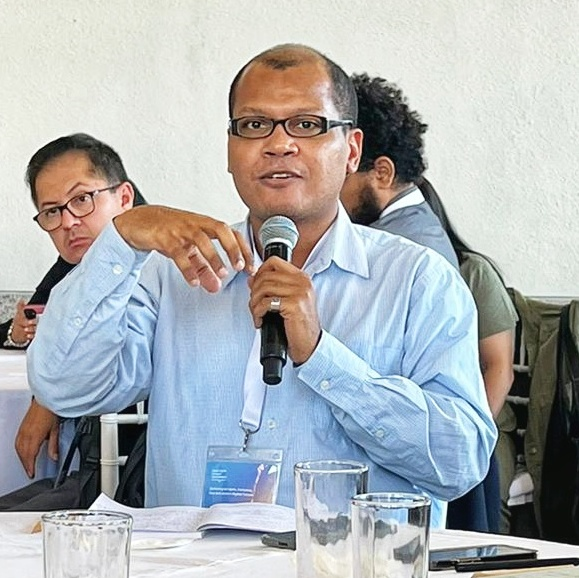
\includegraphics[width=0.4\linewidth]{content/mexican_nlp/umut.png}

\textbf{\daydateyear{}, 14:30--15:30 CST}\\
\textbf{Do\~na Adelita}
\end{center}

\noindent
{\bfseries Abstract:}
We will explore the synergy between open data and collaborative construction with a gender lens, unraveling how this combination becomes a fundamental catalyst for the creation of more equitable and bias-free deep language models. We will take a close look at how the transparency and accessibility of open data, along with the active inclusion of gender perspectives in its construction, contribute significantly to mitigating inherent biases in LLMs. We will see how the use of practical strategies demonstrate how this approach not only addresses crucial challenges, but also drives innovation towards a future where NLPs and LLMs more accurately and fairly reflect the diversity of our society. In conclusion, we propose a path towards collaboratively building a more inclusive and equitable technological future.

\vspace{1em}

{\bfseries Biography:}
Umut Pajaro Velasquez holds a BA in Communications and, an MA in Cultural Studies. Now is an Information Systems Ph.D.~student. Currently delving into digital rights and AI ethics, striving to rectify biases, particularly those affecting gender, race, and marginalized communities in technology. Actively contributor and advocator to global dialogues on digital governance. As former Chair of the ISOC Gender Standing Group, they have spoken at events like the Internet Governance Forum and RightsCon. Their involvement includes roles such as a Mozilla Festival Wrangler, Lideres LACNIC 2.0, and Open Life Science 7 Fellow. They are a published researcher in mass media, digital rights, and AI ethics, aiming to transition into academia or diplomacy, and also driven by a passion for photography and poetry.

\newpage
